%% BioMed_Central_Tex_Template_v1.06
%%                                      %
%  bmc_article.tex            ver: 1.06 %
%                                       %

%%IMPORTANT: do not delete the first line of this template
%%It must be present to enable the BMC Submission system to
%%recognise this template!!

%%%%%%%%%%%%%%%%%%%%%%%%%%%%%%%%%%%%%%%%%
%%                                     %%
%%  LaTeX template for BioMed Central  %%
%%     journal article submissions     %%
%%                                     %%
%%          <8 June 2012>              %%
%%                                     %%
%%                                     %%
%%%%%%%%%%%%%%%%%%%%%%%%%%%%%%%%%%%%%%%%%


%%%%%%%%%%%%%%%%%%%%%%%%%%%%%%%%%%%%%%%%%%%%%%%%%%%%%%%%%%%%%%%%%%%%%
%%                                                                 %%
%% For instructions on how to fill out this Tex template           %%
%% document please refer to Readme.html and the instructions for   %%
%% authors page on the biomed central website                      %%
%% http://www.biomedcentral.com/info/authors/                      %%
%%                                                                 %%
%% Please do not use \input{...} to include other tex files.       %%
%% Submit your LaTeX manuscript as one .tex document.              %%
%%                                                                 %%
%% All additional figures and files should be attached             %%
%% separately and not embedded in the \TeX\ document itself.       %%
%%                                                                 %%
%% BioMed Central currently use the MikTex distribution of         %%
%% TeX for Windows) of TeX and LaTeX.  This is available from      %%
%% http://www.miktex.org                                           %%
%%                                                                 %%
%%%%%%%%%%%%%%%%%%%%%%%%%%%%%%%%%%%%%%%%%%%%%%%%%%%%%%%%%%%%%%%%%%%%%

%%% additional documentclass options:
%  [doublespacing]
%  [linenumbers]   - put the line numbers on margins

%%% loading packages, author definitions

%\documentclass[twocolumn]{bmcart}% uncomment this for twocolumn layout and comment line below
\documentclass{bmcart}

%%% Load packages
%\usepackage{amsthm,amsmath}
%\RequirePackage{natbib}
%\RequirePackage[authoryear]{natbib}% uncomment this for author-year bibliography
%\RequirePackage{hyperref}
\usepackage[utf8]{inputenc} %unicode support
\usepackage{graphicx}
%\usepackage[applemac]{inputenc} %applemac support if unicode package fails
%\usepackage[latin1]{inputenc} %UNIX support if unicode package fails


%%%%%%%%%%%%%%%%%%%%%%%%%%%%%%%%%%%%%%%%%%%%%%%%%
%%                                             %%
%%  If you wish to display your graphics for   %%
%%  your own use using includegraphic or       %%
%%  includegraphics, then comment out the      %%
%%  following two lines of code.               %%
%%  NB: These line *must* be included when     %%
%%  submitting to BMC.                         %%
%%  All figure files must be submitted as      %%
%%  separate graphics through the BMC          %%
%%  submission process, not included in the    %%
%%  submitted article.                         %%
%%                                             %%
%%%%%%%%%%%%%%%%%%%%%%%%%%%%%%%%%%%%%%%%%%%%%%%%%


%\def\includegraphic{}
%\def\includegraphics{}



%%% Put your definitions there:
\startlocaldefs
\endlocaldefs


%%% Begin ...
\begin{document}

%%% Start of article front matter
\begin{frontmatter}

\begin{fmbox}
\dochead{Research}

%%%%%%%%%%%%%%%%%%%%%%%%%%%%%%%%%%%%%%%%%%%%%%
%%                                          %%
%% Enter the title of your article here     %%
%%                                          %%
%%%%%%%%%%%%%%%%%%%%%%%%%%%%%%%%%%%%%%%%%%%%%%

\title{Avoidable mortality caused stagnation and reversal in survival improvements among adults in Mexican states, 1990-2015}

%%%%%%%%%%%%%%%%%%%%%%%%%%%%%%%%%%%%%%%%%%%%%%
%%                                          %%
%% Enter the authors here                   %%
%%                                          %%
%% Specify information, if available,       %%
%% in the form:                             %%
%%   <key>={<id1>,<id2>}                    %%
%%   <key>=                                 %%
%% Comment or delete the keys which are     %%
%% not used. Repeat \author command as much %%
%% as required.                             %%
%%                                          %%
%%%%%%%%%%%%%%%%%%%%%%%%%%%%%%%%%%%%%%%%%%%%%%

\author[
   addressref={aff1},                   % id's of addresses, e.g. {aff1,aff2}
   corref={aff1},                       % id of corresponding address, if any
   %noteref={n1},                        % id's of article notes, if any
   email={jmaburto@health.sdu.dk}   % email address
]{\inits{JMA}\fnm{Jos\'e Manuel} \snm{Aburto}}
\author[
   addressref={aff2},
   noteref={n1},
   email={riffe@demogr.mpg.de}
]{\inits{TR}\fnm{Tim} \snm{Riffe}}

%%%%%%%%%%%%%%%%%%%%%%%%%%%%%%%%%%%%%%%%%%%%%%
%%                                          %%
%% Enter the authors' addresses here        %%
%%                                          %%
%% Repeat \address commands as much as      %%
%% required.                                %%
%%                                          %%
%%%%%%%%%%%%%%%%%%%%%%%%%%%%%%%%%%%%%%%%%%%%%%

\address[id=aff1]{%                           % unique id
  \orgname{Department of Public Health \& Max Planck Odense Center on the Biodemography of Aging at University of Southern Denmark}, % university, etc
  \street{J.B. Winsl{\o}ws Vej 9},                     %
  \postcode{5000}                                % post or zip code
  \city{Odense},                              % city
  \cny{Denmark}                                    % country
}
\address[id=aff2]{%
  \orgname{Max Planck Institute for Demographic Research},
  \street{ Konrad-Zuse-Stra{\ss}e 1},
  \postcode{18057}
  \city{Rostock},
  \cny{Germany}
}

%%%%%%%%%%%%%%%%%%%%%%%%%%%%%%%%%%%%%%%%%%%%%%
%%                                          %%
%% Enter short notes here                   %%
%%                                          %%
%% Short notes will be after addresses      %%
%% on first page.                           %%
%%                                          %%
%%%%%%%%%%%%%%%%%%%%%%%%%%%%%%%%%%%%%%%%%%%%%%

\begin{artnotes}
%\note{Sample of title note}     % note to the article
\note[id=n1]{Equal contributor} % note, connected to author
\end{artnotes}

\end{fmbox}% comment this for two column layout

%%%%%%%%%%%%%%%%%%%%%%%%%%%%%%%%%%%%%%%%%%%%%%
%%                                          %%
%% The Abstract begins here                 %%
%%                                          %%
%% Please refer to the Instructions for     %%
%% authors on http://www.biomedcentral.com  %%
%% and include the section headings         %%
%% accordingly for your article type.       %%
%%                                          %%
%%%%%%%%%%%%%%%%%%%%%%%%%%%%%%%%%%%%%%%%%%%%%%

\begin{abstractbox}



\begin{abstract} % abstract
\parttitle{Background} The 20th century was marked by sizable improvements in mortality, living conditions and health in most Latin American countries. 
In Mexico, these improvements have slowed down recently as a result of opposing
trends in particular causes of death.
\parttitle{Methods} We analyze trends in mortality for three large age groups from 1990 to 2015 for all 32 Mexican states, and compare these with a low mortality benchmark. We use the concept of avoidable mortality and apply demographic measures and use standard decomposition techniques to disentangle age-cause-specific effects on survival.
\parttitle{Results} We find improvements in survival for the population below age 15. However, the adult population aged 15 to 39 shows deterioration among males after 2006 in almost every state as a result of an increase in homicide mortality. Adults aged 40 to 74 show an unexpected decrease in the low mortality benchmark, indicating universal deterioration. State-specific departures from this benchmark was caused by ischemic heart diseases, diabetes, cirrhosis and homicide mortality. We find large health disparities between states, particularly for the adult population and specially after 2005.
\parttitle{Conclusions} Mexico has succeeded in reducing mortality and inequalities in children and the young population. Nevertheless, our results show that older adults are becoming a vulnerable group, and more efforts are required to reduce the burden of conditions amenable to health services and policy-related conditions.
%\parttitle{Second part title} %if any
%Text for this section.
\end{abstract}

%%%%%%%%%%%%%%%%%%%%%%%%%%%%%%%%%%%%%%%%%%%%%%
%%                                          %%
%% The keywords begin here                  %%
%%                                          %%
%% Put each keyword in separate \kwd{}.     %%
%%                                          %%
%%%%%%%%%%%%%%%%%%%%%%%%%%%%%%%%%%%%%%%%%%%%%%

%to think about
\begin{keyword}
\kwd{Latin America}
\kwd{health inequalities}
\kwd{adult health}
\kwd{causes of death}
\kwd{homicides}
\kwd{ischemic heart diseases}
\kwd{diabetes}
\kwd{cirrhosis}
\end{keyword}

% MSC classifications codes, if any
%\begin{keyword}[class=AMS]
%\kwd[Primary ]{}
%\kwd{}
%\kwd[; secondary ]{}
%\end{keyword}

\end{abstractbox}
%
%\end{fmbox}% uncomment this for twcolumn layout

\end{frontmatter}

%%%%%%%%%%%%%%%%%%%%%%%%%%%%%%%%%%%%%%%%%%%%%%
%%                                          %%
%% The Main Body begins here                %%
%%                                          %%
%% Please refer to the instructions for     %%
%% authors on:                              %%
%% http://www.biomedcentral.com/info/authors%%
%% and include the section headings         %%
%% accordingly for your article type.       %%
%%                                          %%
%% See the Results and Discussion section   %%
%% for details on how to create sub-sections%%
%%                                          %%
%% use \cite{...} to cite references        %%
%%  \cite{koon} and                         %%
%%  \cite{oreg,khar,zvai,xjon,schn,pond}    %%
%%  \nocite{smith,marg,hunn,advi,koha,mouse}%%
%%                                          %%
%%%%%%%%%%%%%%%%%%%%%%%%%%%%%%%%%%%%%%%%%%%%%%

%%%%%%%%%%%%%%%%%%%%%%%%% start of article main body
% <put your article body there>

%%%%%%%%%%%%%%%%
%% Background %%

\section*{Background}
The 20th century was marked by sizable improvements in mortality, living
conditions and health in most Latin American countries \cite{who2000}. 
In Mexico, these improvements have slowed down recently as a result of opposing
trends in particular causes of death. For instance, homicide and diabetes
increased during the first decade of the 2000's, even as infectious and
respiratory diseases continued to fall over the same period. While life
expectancy at birth increased by 4.3 years for males (from 67.6 to 71.9) and 3.4
for females (from 73.8 to 77.2) between 1990 and 2000 \cite{SOMEDE},
between 2000 and 2010, life expectancy at birth entered into a period of
stagnation for males and slowed progress for females \cite{canudas2014}. 


This
period coincides with the implementation of different public health
interventions, such as the Universal Vaccination Program and Seguro
Popular, which aim to provide primary and secondary
health care to the uninsured population and allocate funds to cover catastrophic
health expenditures \cite{knaul2005}. Further, conditional cash transfer programs were introduced to supply incentives for families to reinvest in education, health, and nutrition in 1997 \cite{neufeld2012}. Some evidence
suggests that Mexico experienced substantial decreases in infant and child
mortality, along with improvements that contributed to the reduction of
mortality and in the prevalence of acute malnutrition between 1980 and 2000
because of these interventions \cite{sepulveda2006}. Similarly, by 2012 Seguro Popular had provided health insurance coverage to an additional 52 million
people in Mexico that previously did not have any access to public health care and, as a result, there has been a reduction in catastrophic health expenditures \cite{knaul2012}.

These actions underscore broad progress in public health interventions, but they mask heterogeneity between Mexican states and the epidemiological patterns for different age groups. Therefore, it is necessary to assess the varied impacts that these interventions may have had on mortality in Mexican states \cite{urquieta2015evolution}. For instance, conditional cash transfers are focused on the poorest states, and Seguro Popular was introduced at different times in different states. In addition, Mexico faces a rapid aging process in which we can anticipate the interaction between infectious diseases and noncommunicable conditions \cite{Bygbjerg1499} on the adult population.\footnote{The percentage of the population aged 60 or older is projected to go from 10\% in 2015 to 15\% in 2030 \cite{CONAPO}.} Identifying specific opportunities to improve and put forward solutions to reduce the gap of  the unequal impact of public health interventions on health is a necessary step to promote equitable increases in survival among the Mexican population.% the high degree of social and health inequalities present in the country \cite{Frenk2006} 
% In addition,  given the improvements in health care coverage, the strong role %of institutions, and ongoing public
 %health interventions, 
 
 One approach to assess the impact of health care and other interventions is by operationalizing the
 concept of Avoidable or Amenable Mortality (hereafter abbreviated AM)
 \cite{nolte&mckee2004, nolte&mckee2008,elo2014}. This categorization of mortality aims to measure the quality of health service systems by selecting certain
 causes of death that should not occur in the presence of effective and
 timely health care. Among industrialized countries, such as United States,
 Australia, France, Japan, a reduction in AM rates was
 observed over the past 20 years
 \cite{nolte&mckee2008}. Avoidable mortality rates fell, on average, by 17\%
 for males and 14\% for females in these countries. Despite mortality reductions from cancers and circulatory diseases for
 both sexes, heterogeneity between countries persists, with the United
 States showing the smallest reductions (around 5\%) for both sexes  \cite{nolte&mckee2008}. 
 
 In Mexico, the components of avoidable mortality had different trends since the
late 1990's. Between 2000 and 2004 AM decreased, particularly from
infectious diseases and nutrition-related conditions \cite{francomarina2006}, while it increased between 1998 and 2010 due to diabetes, circulatory diseases, perinatal and respiratory conditions
\cite{agudelo2014efecto}. Increases in the latter causes
of death were particularly concentrated in the poorest states of the country
\cite{davila2014mortalidad}. We aim to extend these studies
by a more focused segmentation of AM into health intervention-related AM and
behavior-related AM. Also, we extend analysis to all 32 states, by sex, and over
the full 26-year period from 1990 to 2015. Finally, we compare state mortality patterns
with an easy-to-understand low-mortality benchmark calculated for large age groups (e.g., 0-14, 15-39, 40-75). This low mortality
benchmark is calculated on the basis of the lowest observed mortality within
ages and causes, selected from the full set of 32 Mexican states. This concept has been previously used in mortality studies \cite{whelpton1947}, and further developed elsewhere 
\cite{wunsch1975minimum,vallin2008minimum}. Deviations from the low-mortality benchmark indicate a strong potential for improvement. We apply demographic measures and
standard decomposition techniques to isolate the cause and age-specific deviations between states and the low mortality optimal lifetable for each year.

We hypothesize age-dependent variations in mortality outcomes.
In particular, we expect convergence between states and improvement in survival
for young people, since public health interventions are mainly focused in infant
mortality and child health. For instance, the vaccination program and the health
reform aim to fully cover children in the entire country, and recent
evidence suggests a decrease in mortality between ages 0 to 14 due to a decline
in infectious and respiratory diseases \cite{gonzalez2016mexico}. On the contrary, we
expect little improvements in survival for the  young-adult population due to the unprecedented rise in homicide mortality, and among older adults because of the increase in diabetes along with endocrine/metabolic diseases in these ages in the country \cite{gonzalez2011health,gonzalez2016mexico}. Although every
state has the commitment to provide universal coverage and equitable access to
health care, we anticipate disparities between states
in mortality improvements due to state differences in epidemiological patterns  \cite{gomez2016dissonant} and differences in how  health care programs have been delivered to the population
\cite{Frenk2006}.


\section*{Data \& Methods} 
Our analyses are based on publicly available anonymized datasets. We used deaths microdata available from official files produced by the
Mexican Statistical Office from 1990 to 2015 \cite{INEGI}. These data contain
information on causes of death by single age, sex, and state of residence at the
time of death. Population estimates from 1990 to 2015 came from the Mexican Statistical Office as well \cite{INEGI}. These estimates adjust for age misstatement, undercounting, and interstate and international migration. Death counts and estimated of the population exposed to risk were used to calculate cause-age-specific death rates by sex and state from 1990 to 2015.

\subsection*{Classification of Causes of Death}

To separate causes of death that are susceptible to medical intervention (such as
infectious and respiratory diseases) and those related to health behaviors and
specific public policies (such as homicides, lung cancer) we use the concept of
``Avoidable/Amenable Mortality'' (AM) \cite{nolte&mckee2004, nolte&mckee2008}. We group causes of death into ten categories based on a previous classification  \cite{elo2014} that has recently been adapted to the case of Mexico \cite{Aburto2015}. Table~\ref{tab:causes} lists the cause of death categories we use with relative frequencies by sex for the period 2000-2015.



We separate diabetes, ischemic heart diseases (IHD), HIV/AIDS, lung
cancer, and cirrhosis because these causes are susceptible to both health behavior
and medical service, and because the first two represent major causes of death
in Mexican adults \cite{gomez2016dissonant}. We also separate
homicide, road traffic accidents, and suicide because they have emerged as
leading causes of death among young people, and the first two recently had a sizeable
impact on life expectancy recently in Mexico \cite{Aburto2015}. All causes of death were classified using the International Classification of Diseases, revision 9 for the period 1990-1997 and the tenth revision for 1998-2015 (see SI Table 1 for details on ICD codes for each cause). For the sake of a continuous cause of death series from ICD-9 to ICD-10, we grouped specific causes using codes from a previous study on avoidable mortality in the US \cite{elo2014}. To check the validity of these cause of death bridge codes in Mexico, we performed a sensitivity analysis and did not find major changes in mortality trends by AM classification (See SI figure 1). Although ill-defined causes represent a small percentage of the total deaths (2\% in 1992 \cite{rivera2002epidemiological}), we decided to leave them in the residual category rather than redistributing over other causes of death. We suspect that ill-defined causes could be related to specific conditions, such as homicides, in Mexico.

We truncated analysis at age 75 because cause of death classification and age reporting are considered to be inaccurate in death registration at older ages \cite{tobias2001} and most changes in life expectancy are likely due to changes in mortality patterns below the age of 75 \cite{Aburto2015}. This does not mean that the population above age 75 should not be included in public health priorities.

\subsection*{Age Groups}

We break life expectancy into three large age groups to capture mortality differences along the lifespan. The first group refers to people aged 0-14. This group is likely to represent improvements in causes amenable to medical service (e.g. infectious diseases and conditions of perinatal period) \cite{canudas2014}. The second group, aged 15-39, is used to capture the effect of homicide mortality and external causes, historically related to the young-adult mortality jump. This age group had an important impact on changes in state life expectancy in the first decade of the 2000s \cite{Aburto2015}. The third group covers older adults aged 40-74. We focus on older adults because they likely represent a vulnerable group since mortality rates at adult ages deteriorated in recent years from non-communicable diseases and injury-related mortality \cite{gonzalez2011health,gomez2016dissonant}.

\subsection*{Demographic Methods}
We smooth cause-specific death rates over age and time for each
state and sex separately using the 2-d p-spline
to avoid random variations between ages \cite{GC2012}. Smoothed death rates are
then constrained to sum to the unsmoothed all-cause death rates. We then calculate period life tables up to
age 74 for males and females from 1990 to 2015 following standard demographic methods \cite{HMDMP}. We calculate the average years lived in each age group (temporary life expectancy) \cite{arriaga1984} (See SI for a technical overview) and estimate cause-specific contributions to the difference between
state-specific temporary life expectancy and  the low mortality benchmark using
 standard decomposition techniques \cite{horiuchi2008}. Finally, to measure the level of disparities between states over time, we estimate the coefficient of variation and the Gini coefficient on average survival for each age-group in each year. 

\subsection*{Low mortality benchmark}
Our low-mortality benchmark is calculated in the basis of the lowest observed mortality rates by age, cause of death, from among all states for a given sex and year.

The resulting minimum mortality rate schedule has a unique age profile, and it determines our benchmark temporary life expectancy. The minimum mortality schedule can be treated as the best presently achievable mortality assuming perfect diffusion of the best available practices and technologies in Mexico \cite{vallin2008minimum}. This value is a practical reference because it is based neither on a projection of improvements into the future nor on an arbitrary and likely dissimilar population. 


\subsection*{Limitations}
Mortality data from Mexico are
likely to present inaccuracies in cause-of-death classification due to
comorbidities, particularly at older ages \cite{tobias2001}. To mitigate this,
we focus on ages below 75 and grouped causes of death using ICD codes.
Our estimates regarding homicide mortality are likely to be
underestimated due to inaccurate practices regarding counting, reporting,
and due to the large number of missing individuals in Mexico \cite{HRW2011}.

Avoidable mortality should be understood as an indicator of potential
weaknesses with respect to health care and some public health policies and not
as a definitive assessment \cite{nolte&mckee2008}.

The amount of deaths that should be considered avoidable within the avoidable classification is not clear \cite{beltran2011avoidable}. For instance, some researchers consider only 50 percent of heart disease mortality to be avoidable \cite{nolte2012amenable, holland2003}. We do not have information to precisely
measure percentages of avoidable mortality within cause groups in Mexico. Nonetheless, the
difference between a given mortality schedule and the best mortality schedule of
the same year can be conceived of as a minimal definition of avoidable
mortality. The benchmark mortality schedule sets a lower bound to how much mortality could have been avoided. Certainly, even the best mortality schedule will contain elements of mortality that
most would consider avoidable. To the extent that the components of the benchmark schedule were indeed
attained somewhere in Mexico, one can view any excess mortality
with respect to the benchmark schedule as avoidable. We believe this perspective improves on the AM concept by giving a directly measurable standard against which to estimate avoidable deaths.

\section*{Results}

\subsection*{Trends in mean survival for Mexican states by age-groups}

Figure \ref{Fig1} presents average survival (temporary life expectancy) by state  for three large age groups, young (ages 0-14), young adults (15-39) and older adults (40-74), over the period 1990-2015. Grey lines refer to each one of the 32 states; and the blue lines represent the low mortality benchmark. The black line at the top of each panel indicates the maximum survival in each age group. For example, the young group has a maximum of 15 livable years, while young and older adults have 25 and 35, respectively. Any gap between a state line and the blue line represents a potential gain in survival if mortality were to achieve the low mortality benchmark.

All states show improvements in the young age group from 1990 to the early 2000s approaching the low mortality benchmark, which is very close to full survival below age 15. In contrast, Mexico City (former Federal District) has lagged behind in reducing mortality at these ages; and some states, such as Tabasco and Chiapas, even experienced a downward in survival in both sexes in recent years.

Survival among young male adults shows a common shift after 2005 in almost every state in Mexico. In 2005 the male mean survival between states was 24.5 years; by 2010, twenty states were below this number. Chihuahua, Sinaloa and Durango, in the Northern region, experienced substantial losses in 2010, and consequently the largest departures from the low mortality benchmark. In 2015, the states with the lowest survival were Guerrero, Chihuahua and Tabasco. Trend for females were similar, albeit with lower magnitude, with the exception of Chihuaha, which clearly shows a shift after 2005 in survival, comparable to those observed in males.

In older adults, survival shows stagnation and deterioration during the entire period. Even the low mortality benchmark exhibits a gradual downward trend, pointing to small increases in adult mortality in every state. Of a maximum of 35 years, females in the Mexican states were living on average around 32, and men 30.5 in 2015. These values are very close to those observed 10 years earlier, 31.9 and 30.4 respectively. Similar to the young adults, in some states males experienced a  clear downward trend after 2005. Throughout the entire period, the most disadvantaged states were Baja California, Chihuahua and Mexico City. \\

\begin{center}
[Figure \ref{Fig1} about here]
\end{center}


\subsection*{Inequalities in survival by age-groups}
Figure \ref{Fig2} shows survival inequalities for the Mexican states, as measured by the coefficient of variation, by age group (results for the Gini coefficient are reported in SI figure 2). Larger values are related to higher disparities between states. 


Since 1990, survival inequality among the young population has been decreasing. Young adults show even lower inequality than the population at younger ages in both females and males. However, after 2005 the level of disparities begun to increase in males, and by 2007 there was a crossover leading to higher inequality. The highest values are observed in the period 2009-2011. By 2015 the level has not yet recovered, and still is higher than that of the young population.

Older adults show substantially higher inequality than the other age groups in the entire period. Similar to young male adults, after 2005 they experienced an upturn, and a slowly recovery until 2012. From 2013, both males and females show a rise in disparities between states. Survival below age 75 (dotted line) shows a similar trend, although with lower levels. Importantly, women show less inequality in every age group at any year.\\

\begin{center}
[Figure \ref{Fig2} about here]
\end{center}


\subsection*{Causes of death}


In figures \ref{Fig3} and \ref{Fig4}, the Mexican states in each region are arranged according to potential gains in survival for older adults in 2015, i.e. departure of each state from the low mortality benchmark. 

Figure \ref{Fig2} shows how causes amenable to medical service, diabetes, ischemic heart diseases (IHD), lung cancer, cirrhosis, homicide and road traffic accidents contributed to the gap between each state and the low mortality benchmark from 1990 to 2015 for male older adults (ages 40-74). These are the causes of death that contributed the most to impeding the states from achieving the low mortality benchmark. Light-yellow colors indicate no contributions to the gap, which means that are very close to the low mortality benchmark within each category. Darker red hues indicate larger contributions to the gap. If a particular state is improving during the period, it shows a transition from red to light-yellow. 

Medically amenable causes of death show gradual improvements in most states from 1990 to 2015, leading to decreasing the gap with the benchmark in this category. However, large disparities between states and large room for improvements remain. For example, Baja California, Chihuahua, Sonora and Coahuila from the northern region; along with Mexico City; and most states in the south would significantly increase survival by reducing the mortality associated to this category. Mortality caused by diabetes has increasingly contributed to the gap with the benchmark in some states. Coahuila and Tamaulipas in the north; Mexico City, Guanajuato and Tlaxcala in the central region; and Puebla, Veracruz and Tabasco in the south, show deterioration in diabetes mortality in the last decade, leading to widening the gap with the benchmark. Similarly, IHD affects significantly the north part of the country, while cirrhosis is mostly concentrated in the south. Although lung cancer and road traffic accidents do not have the same magnitude as these previous causes, every state would reduce the gap by lowering mortality related to these conditions. Cause specific mortality for homicides shows a clear reversal in improvement trends around 2010. Particularly, Baja California, Chihuahua, Durango and Sinaloa in the north; Colima, Michoacan and Nayarit in the central region; and Morelos and Guerrero in the southern part of the country. Importantly, Oaxaca, Guerrero, Morelos, and other states in the north point towards an upsurge of homicide mortality in 2015. 

\begin{center}
[Figure \ref{Fig3} about here]
\end{center}

Causes amenable to medical service, diabetes and IHD are the causes of death that mostly contribute to the gap with the low mortality benchmark among older adult females (see SI figure 3). Although almost every state shows improvements in causes medically amenable, these conditions still represent potential years of life if the low mortality benchmark were achieved in this age group. Diabetes shows deterioration in recent years in several states, such as Coahuila, Tamaulipas in the north; Guanajuato and Tlaxcala in the central area; and Puebla, Veracruz and Tabasco in the south, among others, widening the gap with the low mortality benchmark. Moreover, IHD contributes significantly to the gap, particularly in the northern region, and there are not clear improvements throughout the entire period 1990-2015.

Among the young population below age 15, improvements in survival and in reducing the gap with the low mortality benchmark were mainly driven by causes amenable to medical service in both females and males. However,  Mexico, Tlaxcala, Mexico City in the central region, along with almost every state from the south still could improve (see SI figures 4 and 5). Finally, the causes of death that mainly explain the trends in the gap with the benchmark on the young male adults (ages 14-39) are homicides and road traffic accidents (see SI figures 6 and 7). States like Chihuahua, Durango, Sinaloa and Guerrero would benefit with an additional year of life in these ages by reducing homicide mortality to the low mortality benchmark. The impact of the remaining  AM categories in ages 0-14 and 15-39 is negligible. \\



\subsection*{Potential gains and causes of death in 2015}

Figure \ref{Fig4} shows the potential gains in survival for male older adults if the low mortality benchmark were achieved for the years 2005 (light blue triangles), 2010 (rhombus) and 2015 (dark blue dot) in the left panel. The right-hand panel shows the proportion of potential gains explained by specific causes of death for 2015.

Every state in Mexico could increase survival by one year in older adult ages if they were to achieve the low mortality benchmark, with the exception of Nayarit, in 2015. Since 2005, no major improvements are clear, and in some states the potential gains even increased in 2015 compared to 2010, for example San Luis Potos\'i and Zacatecas in the north; Colima, Guanajuato, Mexico City in the central region; and all the southern region, with the exception of Guerrero. 

Importantly, in every state more than half of the potential gain is explained by avoidable causes of death, and in some states more than 75\% (righ-hand panel). In particular, causes amenable to medical service, along with mortality related to health behavior, such as diabetes, IHD, cirrhosis, homicide and traffic accidents play an important role in explaining the gap with the low mortality benchmark. Moreover, their relative importance has not changed since 2005 (see SI figure 8).\\

\begin{center}
[Figure \ref{Fig4} about here]
\end{center}


Females show similar results than males but with lower magnitude (see SI figures 9 and 10). However, Baja California, Chihuahua, Sonora, and Coahuila in the northern region; Mexico City in the center; and  Puebla, Veracruz, Tabasco, Yucat\'an, Morelos, Chiapas and Quintana Roo in the south show potential gains larger than one year. The respective results for young and younger adults are shown in SI figures 11-16


\section*{Discussion}
\subsection*{Young survival}

This analysis demonstrates the potential contribution of achieving the low mortality benchmark to improvements in survival. However, it is concerning that the low mortality benchmarks have not been steadily increasing over the period studied. Trends were flat for children, they are experiencing almost full survival before age 15. More worrisome is the common shift after 2005 in adults aged 15-39 and decreasing survival among older adults aged 35-74.

Despite the flattening pattern of the low mortality benchmark in children, our results show that all states in Mexico have improved survival towards this benchmark and to the maximum survival. Causes amenable to medical service are at the heart of such improvements, consistent with decreases in infectious and respiratory diseases associated with public health interventions targeted to children in Mexico previously documented \cite{sepulveda2006}. For example, Puebla and Tlaxcala improved survival over half a year since the 1990's. By 2010 survival was improved so that all states' temporary life expectancy ranged between 14.6 and 14.8 years. We further estimated survival inequalities between states by age group for every year.  Indeed, survival inequality below age 15 was reduced paralleling improvements in survival during the period. In addition, our results are also consistent with advances in coverage for skilled attendance at delivery, which by 2012 remained above 90\% and more than 78\% of children under age one visited the doctor to monitor their development and growth  \cite{urquieta2015evolution}. Moreover, vaccination coverage has been achieved for the entire young population, the success of such public health interventions are in line with our results, underscoring the improvements in survival in the population younger than 15 years associated to the progress detected in health insurance coverage due to vaccination programs and the implementation of the Seguro Popular \cite{urquieta2015evolution}. Although average years lived below 15 has improved, there still exist areas of opportunity to achieve full-survival under age 15 in causes amenable to medical service, mainly in states in the Central and Southern regions of the country. 


\subsection*{Young adults}

Young adults (ages between 15 and 39) show a converging pattern towards the low mortality benchmark in all states just until 2005. A sudden increase in homicide rates widened the gap with the low mortality benchmark by almost four times on average in 2010, relative to the level observed in 2005. Previous research documented losses in the overall life expectancy up to three years in the state of Chihuahua (the bordering state with Texas, USA) and almost two years in Sinaloa, Durango (North) and Guerrero (South) between 2005 and 2010 due to homicides \cite{Aburto2015}. Our findings show that the trend towards the low mortality benchmark was reversed after 2005 due to the increase in homicide mortality, with a peak in 2010-2011. Although homicide rates decreased after 2011, they still are the main cause of death contributing to the gap between the observed survival and the low mortality benchmark in particular states, such as Sinaloa, Durango in the North, Nayarit and Michoac\'an in the cetral region, and Guerrero in the South. These findings underscore the need for effective interventions to reduce homicide mortality, as it still contributes the most to survival shortcomings among the young-adult population and mortality inequality among states. Even ten years after the national security strategy that aimed at reducing drug cartels' operations started and homicides begun to spread all over the country \cite{espinal2015analysis}, the effect of homicide on average survival is appalling. Between-state inequality in female survival was much smaller over the same period.


\subsection*{Older adults}

%In Mexico, since the beginning of the 1990's, adult survival in ages 40-74 deteriorate for males and stagnate for females. Our results help explain on this pattern showing that the low mortality benchmark decreased as a result of state-specific mortality trends and the interaction between specific causes of death. In particular, there are offsetting effects between improvements in causes amenable to medical service, such as infectious and respiratory diseases, and deterioration in diabetes, isquemic heart diseases (IHD), and behavior-related mortality through cirrhosis and homicides. 

%Out of 35 potential years, adult females in Mexico are living less than 33 and males less than 31 since the 1990's. The increase in  diabetes, IHD and cirrhosis mortality is at the heart of survival's deterioration, with clear regional variations. Although improvements in causes amenable to medical service were witnessed, almost every state still has potential to improve in this ages, in particular the Northern states of Sonora, Chihuahua and Baja California. Diabetes mortality increased over the period and contributed to increases in the gap to achieve the low mortality benchmark. Diabetes-related mortality increased 23\% from 1998 to 2002, and the prevalence of diabetes was estimated at 14.4\% in the adult population in 2006. These figures underscore the emerging epidemic of diabetes \cite{glassman2010confronting}. To put this in perspective, Coahuila, the state of Mexico, Guanajuato, the Federal District, Tabasco and Puebla could increase survival by almost one year if diabetes mortality were to achieve the low mortality benchmark. Similarly, mortality related to IHD contributes to lowering life expectancy in adults. There is a clear regional pattern in the country. Almost all the states in the Northern region could potentially benefit with one additional year in life expectancy if the low mortality benchmark were reached, where as the Central and Southern regions present a lower impact of IHD. Cirrhosis-related mortality shows a higher impact in the Southern and Central states of the country, particularly in Quer\'etaro, M\'exico state, Hidalgo (central area) and Puebla and Oaxaca in the South. Both diabetes and IHD mortality are closely related to obesity prevalence, previous research anticipated that the increasing levels of obesity in Mexico could compromise gains in life expectancy \cite{monteverde2010obesity}. These regional differences on cause-specific mortality led to increases in health inequalities in adults aged 30-74 after 2006 for males and stagnation among females (figure \ref{fig:Gini}). 


%There is still potential for improvements to reduce state-mortality differences and improve the survival among the adult population in Mexico. Several screening and prevention strategies (e.g. PREVENIMSS) for early diabetes and hypertension have been implemented in the country. However, as previous research has found, they are far from achieving the ultimate goal and including the entire population \cite{castro2010potential}. In addition, \cite{behrman2013health} show that the conditional cash transfer program PROSPERA improves health significantly for adult women older than 50. The authors also noted that the effect on men's health is much lower. They argue that this could be the result of the lack of inclusion of men in the program and the main role of women in the program's requirements. Women are recipients of the monetary transfers and they are more likely to attend clinic visits and follow health measures given by doctors in these clinics than men.\\


\section*{Conclusion}

%Improving health is a priority for governments of many developing countries. In part to reduce child mortality, improve maternal health and lessen the impact of other infectious diseases, such as HIV/AIDS, to achieve the Millennium Development Goals established for 2015 \cite{united2009millennium}.  Mexico has succeeded in reducing mortality and inequalities in children and the young population. Nevertheless, our results show that older adults are becoming a vulnerable group, and more efforts are required to reduce the burden of conditions amenable to health services and policy-related conditions. In particular, this group lacks comprehensive interventions to reduce the burden of violence through homicides, chronic-degenerative causes of death, such as diabetes and IHD, and behavior-related conditions such as cirrhosis.  

%There is no simple way to lessen the impact of such conditions, but it is clear that new approaches are needed to improve survival in the adulthood and to minimize health disparities between states. Preventing diabetes and IHD implies fundamental political challenges. Therefore,  public health initiatives should focus in health care for chronic conditions as recently suggested by \cite{knaul2015achieving}, but they should also influence the population towards improving health behavior. Our results reinforce the need of such, among others public health interventions, with an special focus on older adults in the Mexico. 

%\nocite{oreg,schn,pond,smith,marg,hunn,advi,koha,mouse}

%%%%%%%%%%%%%%%%%%%%%%%%%%%%%%%%%%%%%%%%%%%%%%
%%                                          %%
%% Backmatter begins here                   %%
%%                                          %%
%%%%%%%%%%%%%%%%%%%%%%%%%%%%%%%%%%%%%%%%%%%%%%

\begin{backmatter}

\section*{Competing interests}
  The authors declare that they have no competing interests.

\section*{Author's contributions}
 JMA and TR conceptualized the study, performed the analyses and wrote the manuscript.

\section*{Acknowledgements}
  Text for this section \ldots
%%%%%%%%%%%%%%%%%%%%%%%%%%%%%%%%%%%%%%%%%%%%%%%%%%%%%%%%%%%%%
%%                  The Bibliography                       %%
%%                                                         %%
%%  Bmc_mathpys.bst  will be used to                       %%
%%  create a .BBL file for submission.                     %%
%%  After submission of the .TEX file,                     %%
%%  you will be prompted to submit your .BBL file.         %%
%%                                                         %%
%%                                                         %%
%%  Note that the displayed Bibliography will not          %%
%%  necessarily be rendered by Latex exactly as specified  %%
%%  in the online Instructions for Authors.                %%
%%                                                         %%
%%%%%%%%%%%%%%%%%%%%%%%%%%%%%%%%%%%%%%%%%%%%%%%%%%%%%%%%%%%%%

% if your bibliography is in bibtex format, use those commands:
\bibliographystyle{bmc-mathphys} % Style BST file (bmc-mathphys, vancouver, spbasic).
\bibliography{AburtoRiffe_Bib}      % Bibliography file (usually '*.bib' )
% for author-year bibliography (bmc-mathphys or spbasic)
% a) write to bib file (bmc-mathphys only)
% @settings{label, options="nameyear"}
% b) uncomment next line
%\nocite{label}

% or include bibliography directly:
% \begin{thebibliography}
% \bibitem{b1}
% \end{thebibliography}

%%%%%%%%%%%%%%%%%%%%%%%%%%%%%%%%%%%
%%                               %%
%% Figures                       %%
%%                               %%
%% NB: this is for captions and  %%
%% Titles. All graphics must be  %%
%% submitted separately and NOT  %%
%% included in the Tex document  %%
%%                               %%
%%%%%%%%%%%%%%%%%%%%%%%%%%%%%%%%%%%

%%
%% Do not use \listoffigures as most will included as separate files

\section*{Figures}

\begin{figure}[h!]
\centering
\caption{State-specific average survival (grey lines) and low mortality benchmark (blue line) for young (0-14), young adults (15-39) and older adults (40-74) by sex, 1990-2015.}
\label{Fig1}

%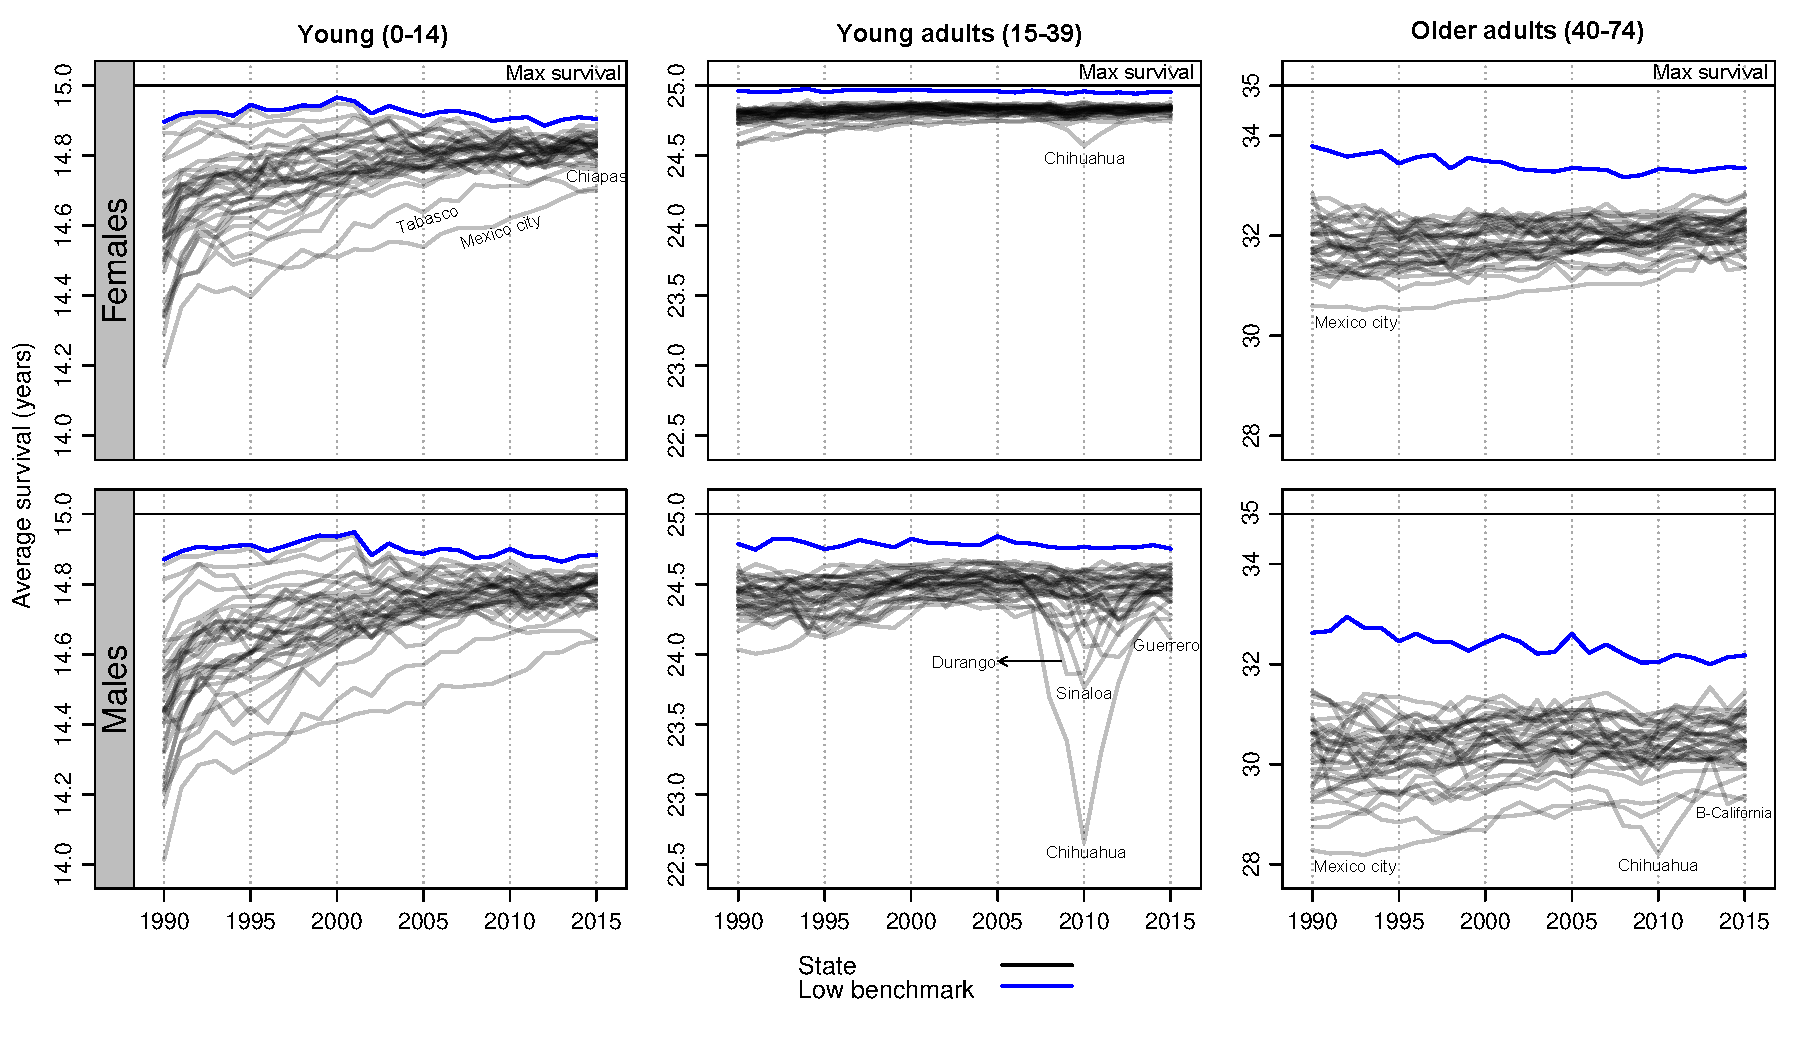
\includegraphics[scale=.35]{Figure1_1.pdf}

Note: Y-axis are not in the same scale in order to capture major trends over the period. Source: calculations based on INEGI files. 
\end{figure}



\begin{figure}[h!]
\centering
\caption{Survival inequality (coefficient of variation) by age group and sex, 1990-2010.}
\label{Fig2}
%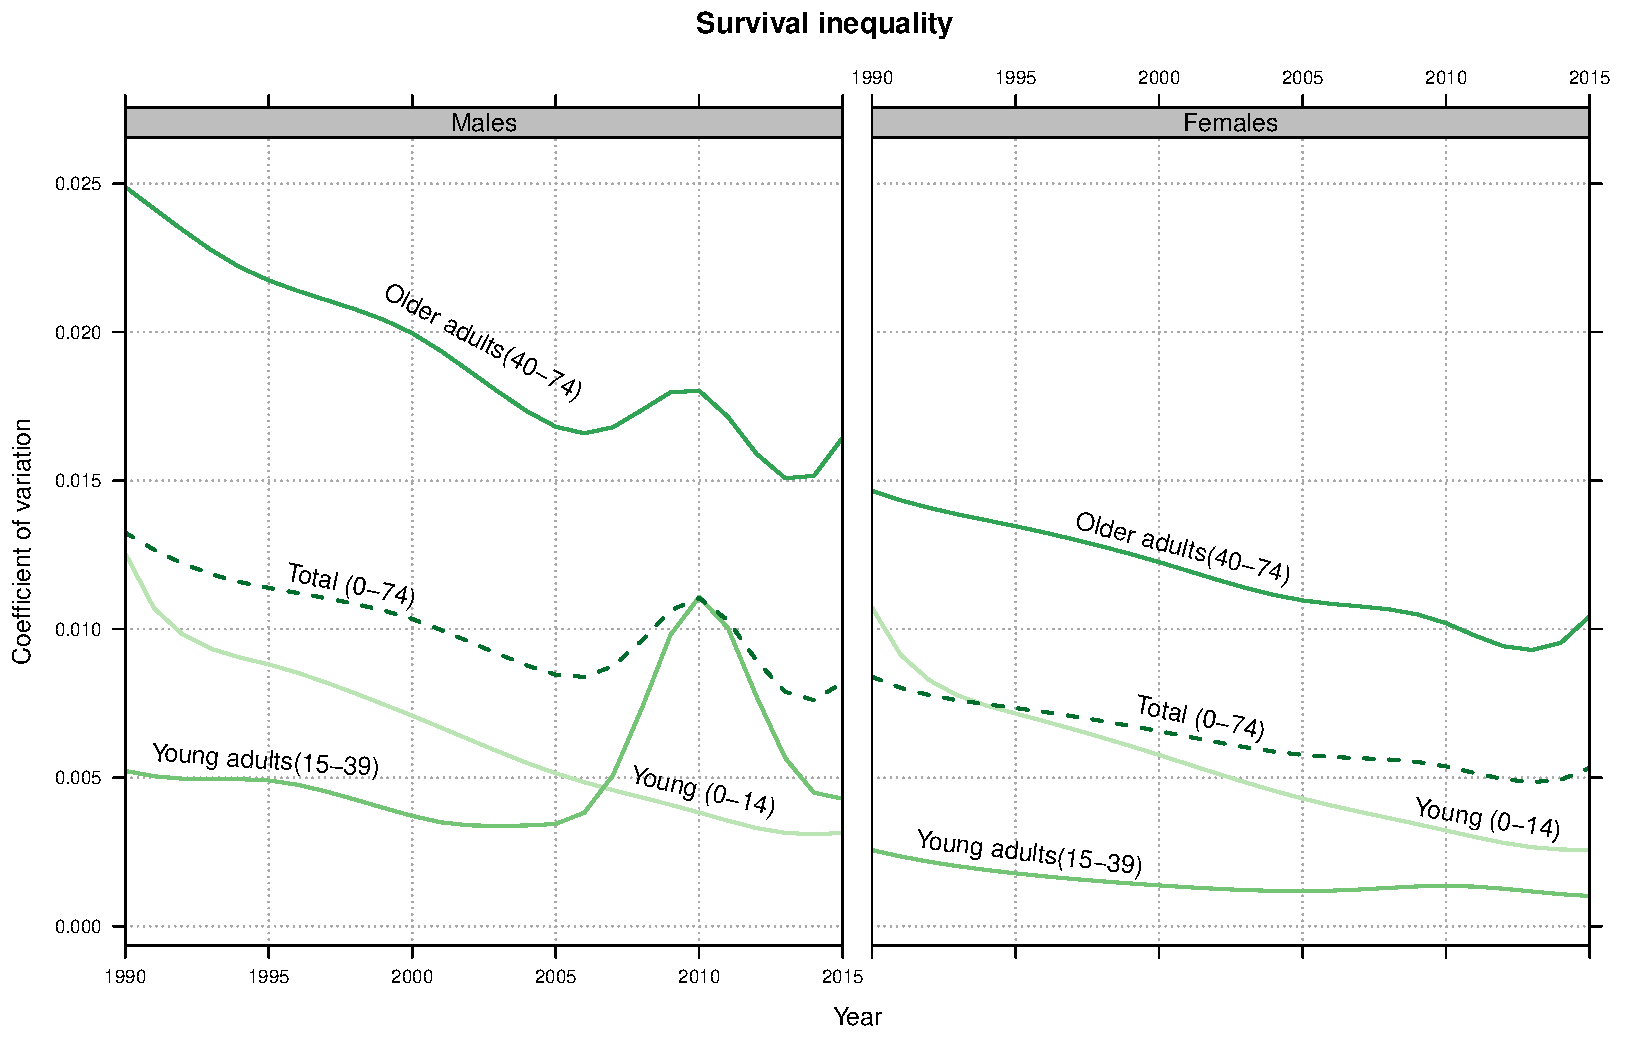
\includegraphics[scale=.4]{CVfig_1.pdf}

Source: calculations based on INEGI files. 
\end{figure}



\begin{figure}[h!]
\centering
\caption{Cause-specific contributions to the gap between state survival and low mortality benchmark for older male adults, 1990-2015.}
\label{Fig3}

%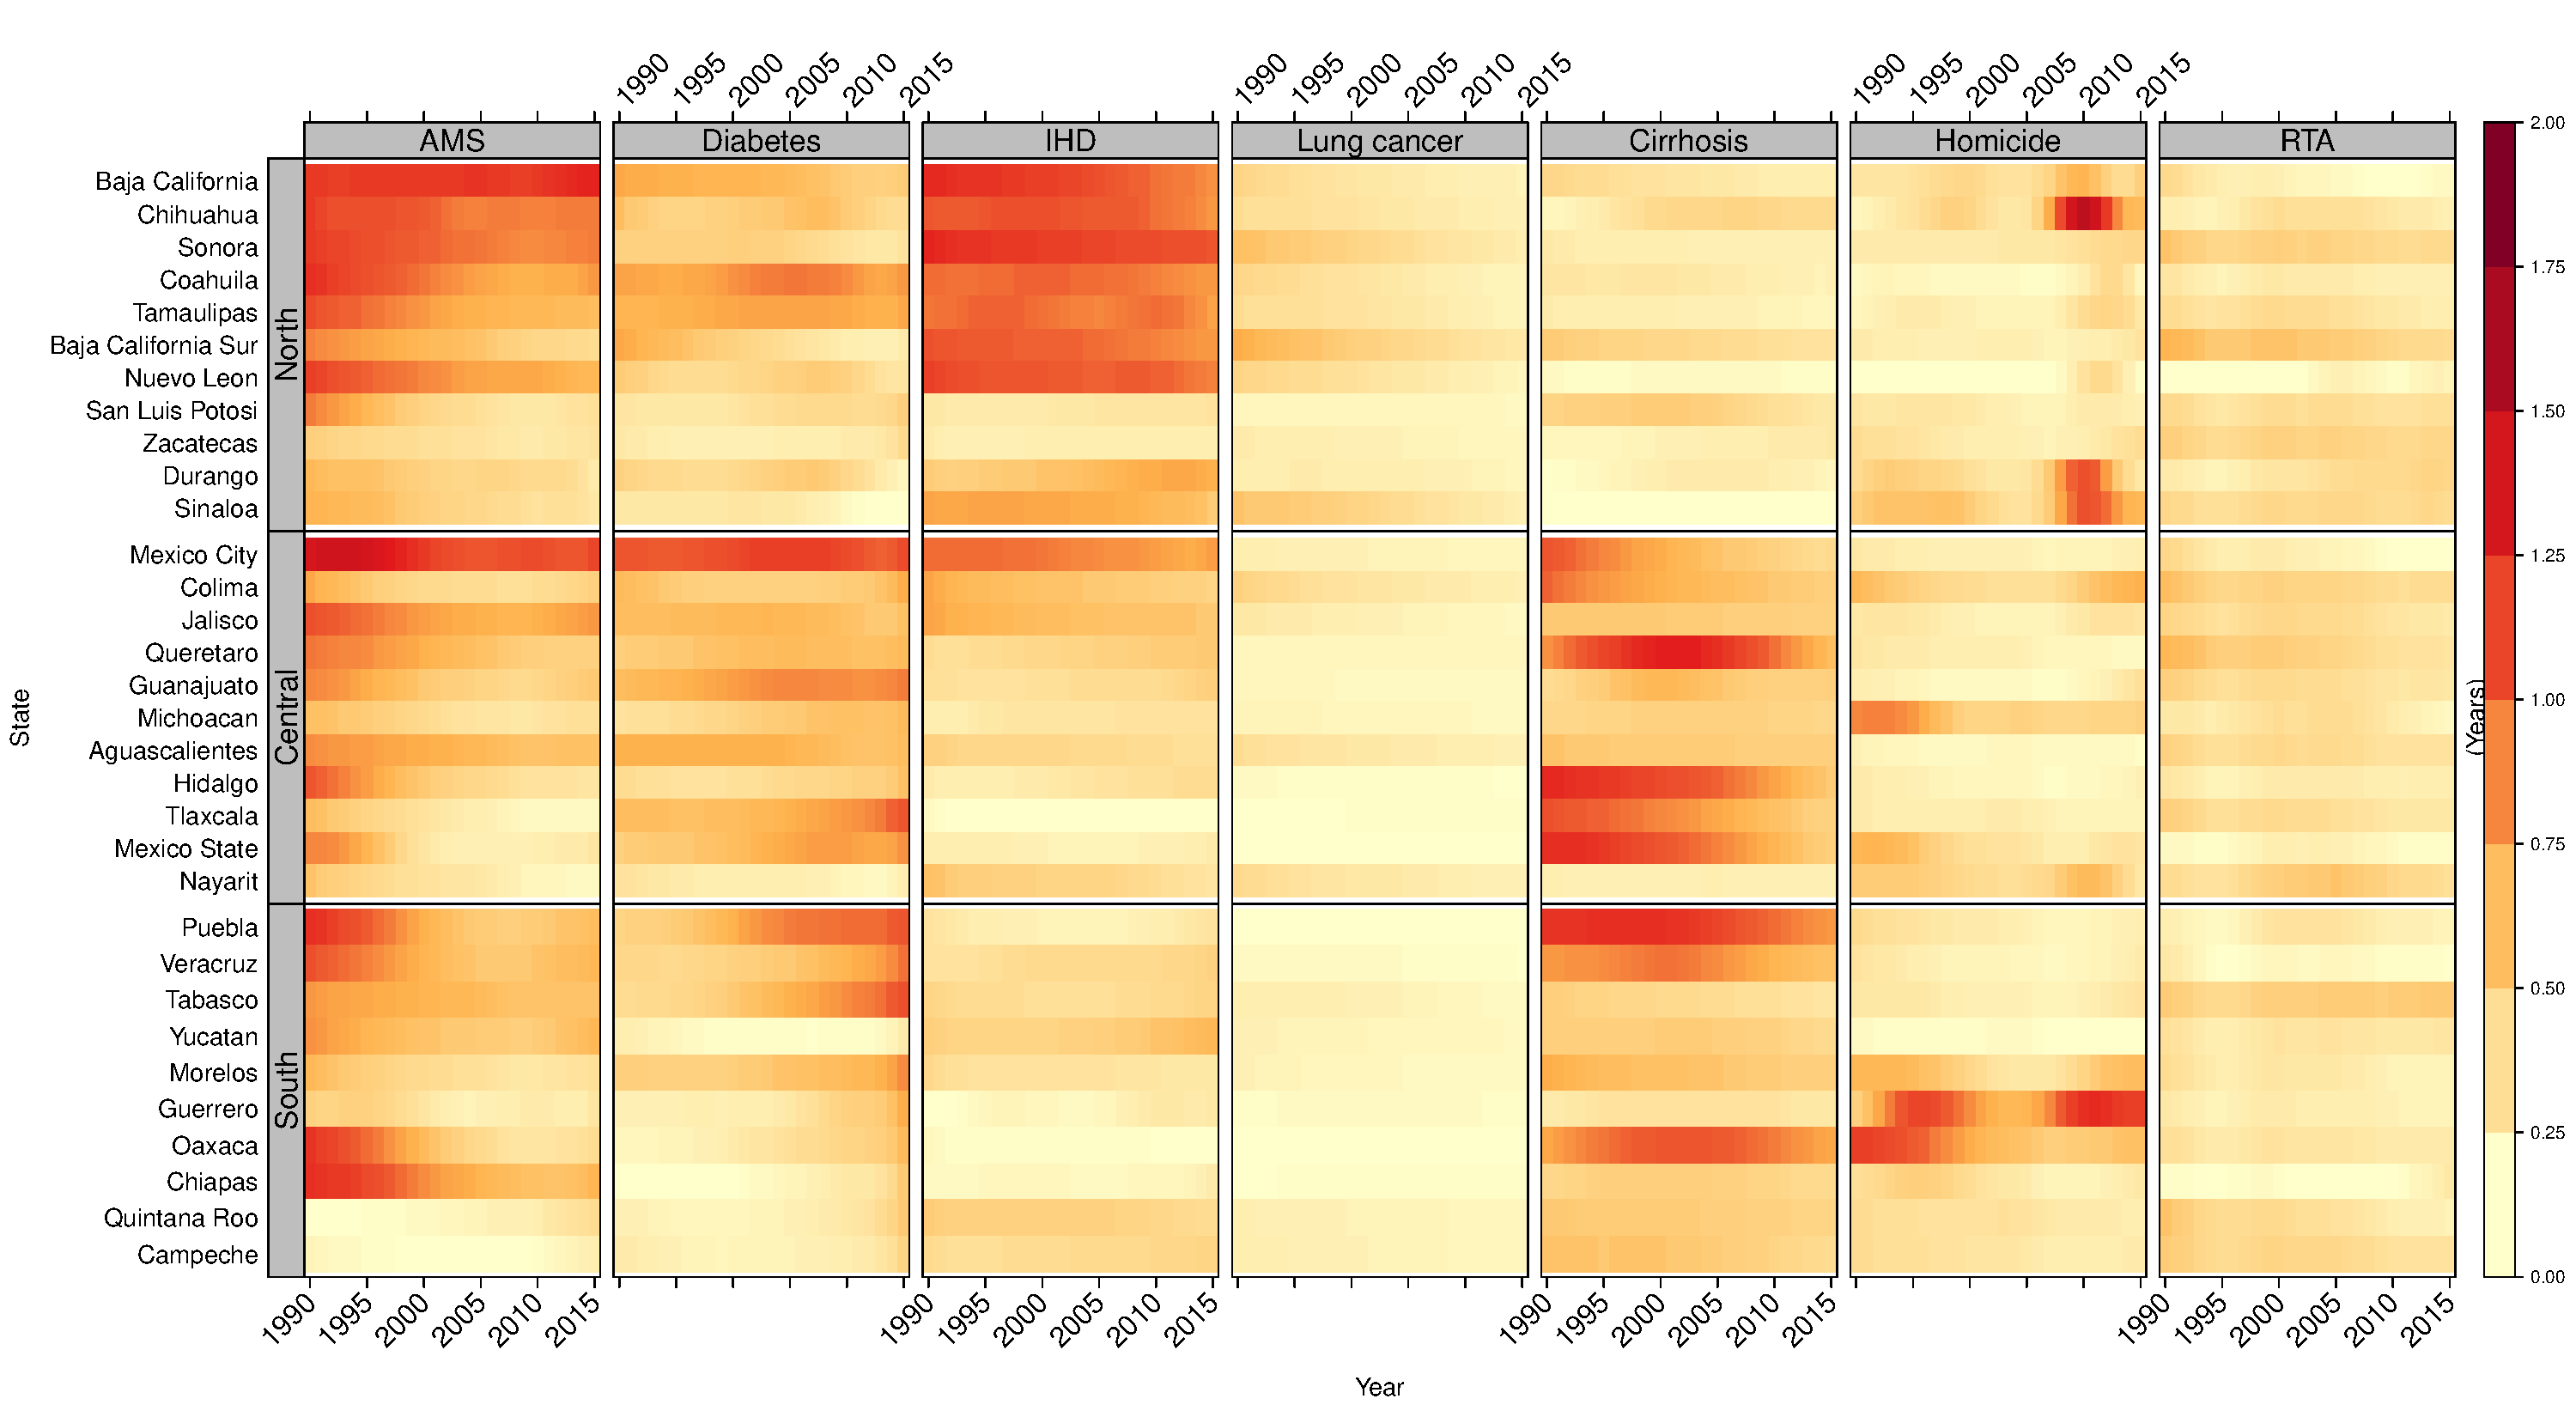
\includegraphics[scale=.23]{AdultMaleheatmap.pdf}

Source: calculations based on INEGI files. 
\end{figure}


\begin{figure}[h!]
\centering
\caption{Left panel: Potential years gained if benchmark were achieved for older adult males in 2005,2010,2015. Right panel: Proportion of potential years explained by cause of death in 2015 }
\label{Fig4}
%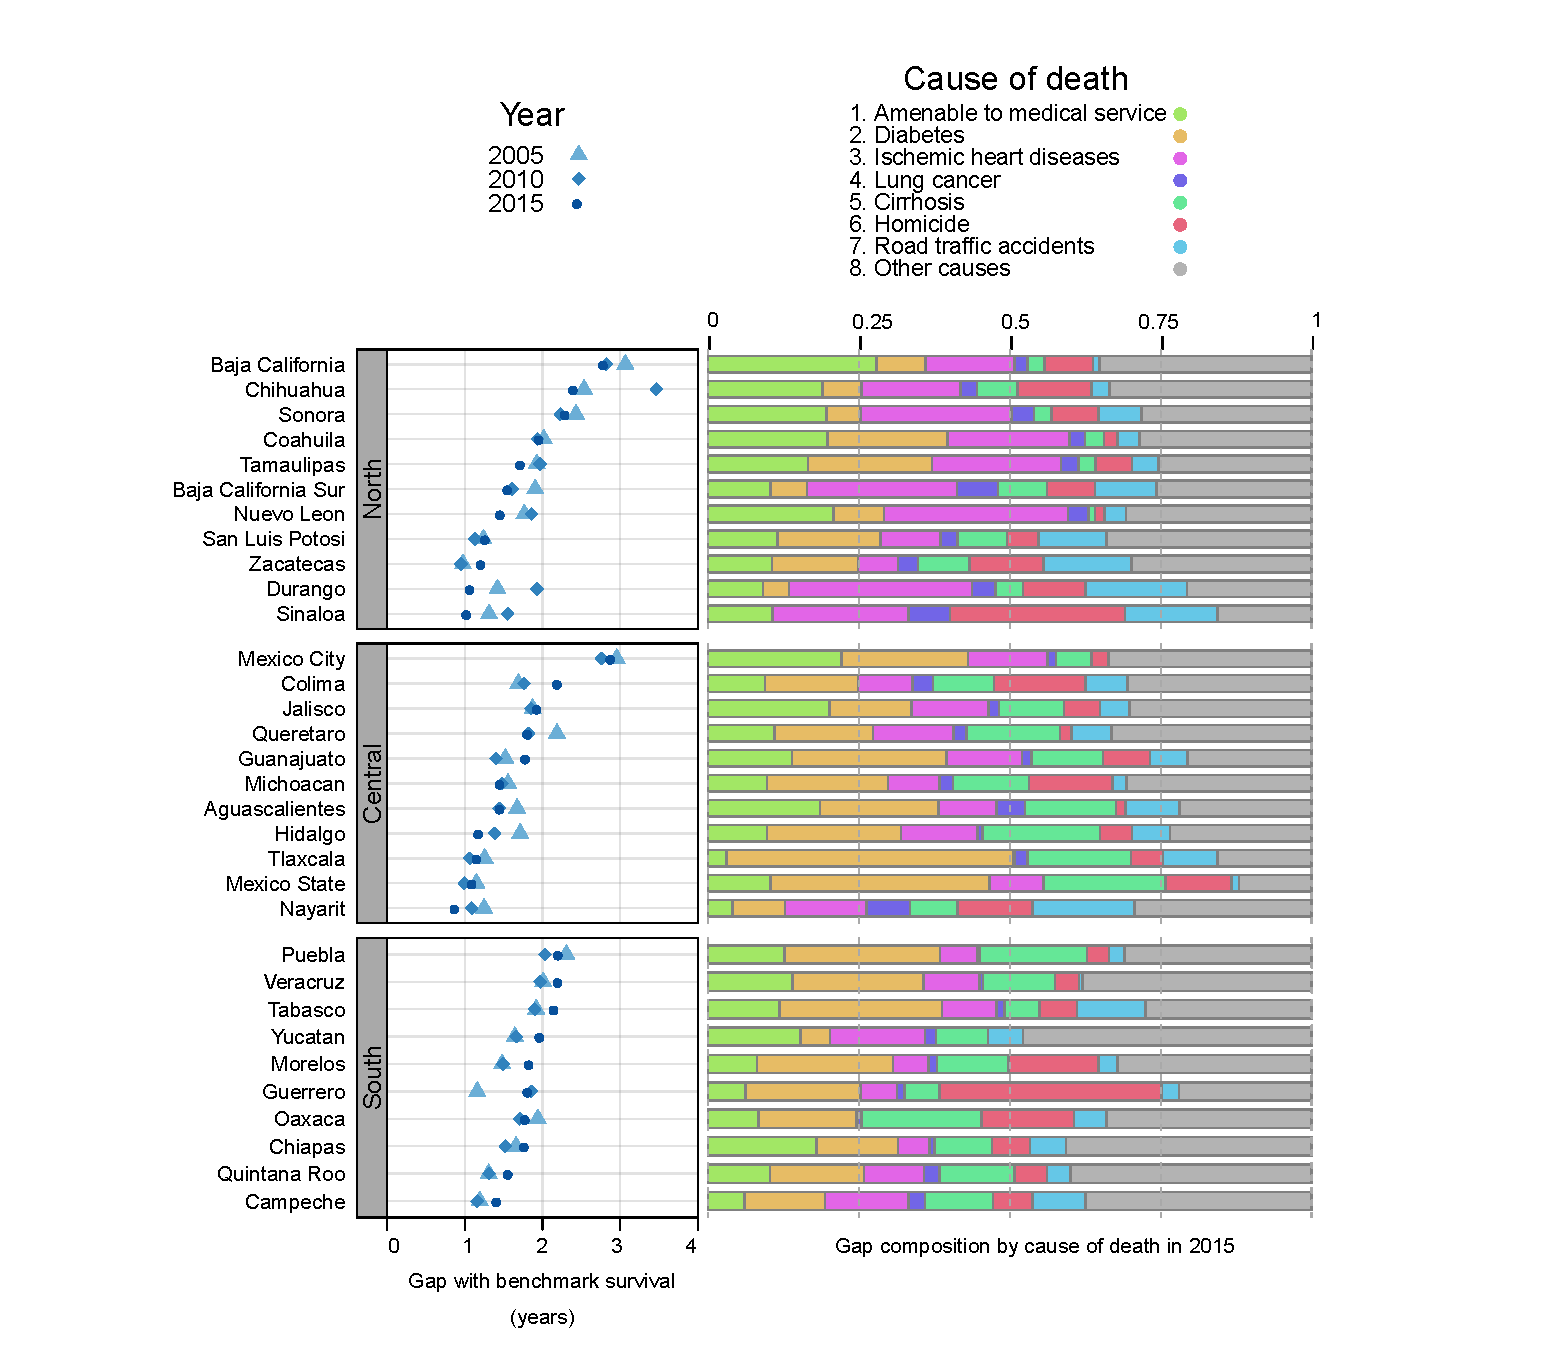
\includegraphics[scale=.45]{Figure_4v2.pdf}

Source: calculations based on INEGI files. 
\end{figure}

%%%%%%%%%%%%%%%%%%%%%%%%%%%%%%%%%%%
%%                               %%
%% Tables                        %%
%%                               %%
%%%%%%%%%%%%%%%%%%%%%%%%%%%%%%%%%%%

%% Use of \listoftables is discouraged.
%%
\section*{Tables}
% latex table generated in R 3.3.1 by xtable 1.8-2 package
% Wed Jan 18 14:53:15 2017
\begin{table}[ht]
\centering
\caption{Avoidable Mortality classification, 
             with crude percentages below age 75, years 1990-2015. Source: INEGI files.} 
\label{tab:causes}
\begin{tabular}{llllll}
  \hline
& Category &\% & Males &  \% & Females \\ 
 &&& (1,000's) & & (1,000's)\\ 
  \hline
1&  Causes amenable to medical service & 30.9 \% & 127.5 & 28.2 \% & 114.4 \\ 
2&  Diabetes & 4.5 \% & 18.7 & 4.9 \% & 19.9 \\ 
3&  Ischemic heart diseases & 4 \% & 16.4 & 4.2 \% & 17 \\ 
4&  HIV/AIDS & 0.4 \% & 1.5 & 0.5 \% & 2.1 \\ 
5&  Lung cancer & 0.9 \% & 3.7 & 0.9 \% & 3.8 \\ 
6&  Cirrhosis & 2.3 \% & 9.5 & 2.5 \% & 10 \\ 
7&  Homicide & 2.7 \% & 11.2 & 3 \% & 12.4 \\ 
8&  Road traffic accidents & 2.8 \% & 11.4 & 2.9 \% & 11.8 \\ 
9&  Suicide & 0.4 \% & 1.7 & 0.5 \% & 1.9 \\ 
10&  Other causes & 24.8 \% & 102.4 & 25 \% & 101.2 \\ 
   \hline
\end{tabular}
\end{table}

%%%%%%%%%%%%%%%%%%%%%%%%%%%%%%%%%%%
%%                               %%
%% Additional Files              %%
%%                               %%
%%%%%%%%%%%%%%%%%%%%%%%%%%%%%%%%%%%

\section*{Additional Files}
  \subsection*{Additional file 1 --- Supplemental material}
   This might refer to a multi-page table or a figure.

  \subsection*{Additional file 2 --- Results}
 Rdata file with all results.


\end{backmatter}
\end{document}
